
This section discusses the performance of the proposed scheduling schemes with the \ac{WSRM} objective. The proposed schemes are compared with the \ac{W-MMSE} scheme which select the users implicitly by forcing the precoder powers to zero when the users are greater than the available \ac{DoF} (overloaded \ac{W-MMSE}). We considered the cell-edge scenario for comparison. The proposed schemes are not optimal when the in-cell users are considered due to the dimensional limitation \me{\mu} discussed earlier which restricts the available \ac{DoF} in the system.
\begin{figure}
\centering
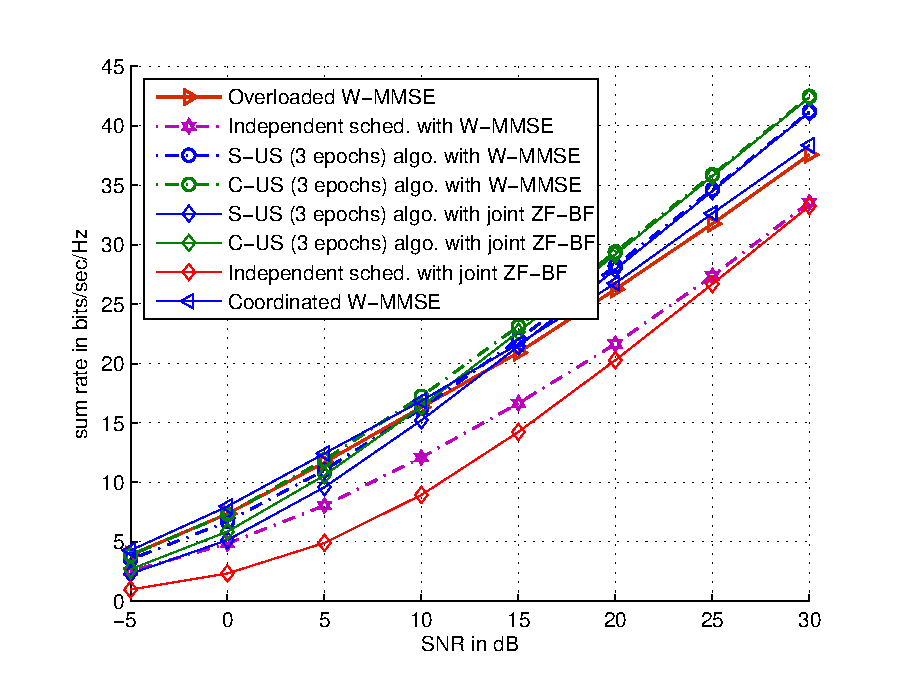
\includegraphics[width=1.0\columnwidth]{multi-bs-1}
\caption[short]{sum rate for \me{N_\mrm{T} = 4, \, N_\mrm{B} = 2, \, \card{\mc{U}_k} = 20}, \, K = 40}
\label{multi-bs-f1}
\vskip -0.2in
\end{figure}

The precoders are designed either with joint \ac{ZF}-\ac{BF} \eqref{sm-e4} or \ac{W-MMSE} scheme \cite{wmmse_shi}. The independent scheduling scheme selects the users independently across each \ac{BS} without any cooperation among \ac{BS}s, but imposes the dimensional constraint \me{\mu} so as to provide interference-free transmission using the precoders. While comparing the scheduling schemes, the \ac{W-MMSE} scheme is used to design the precoders for the users already chosen by the scheduling scheme.
\begin{figure}
\centering
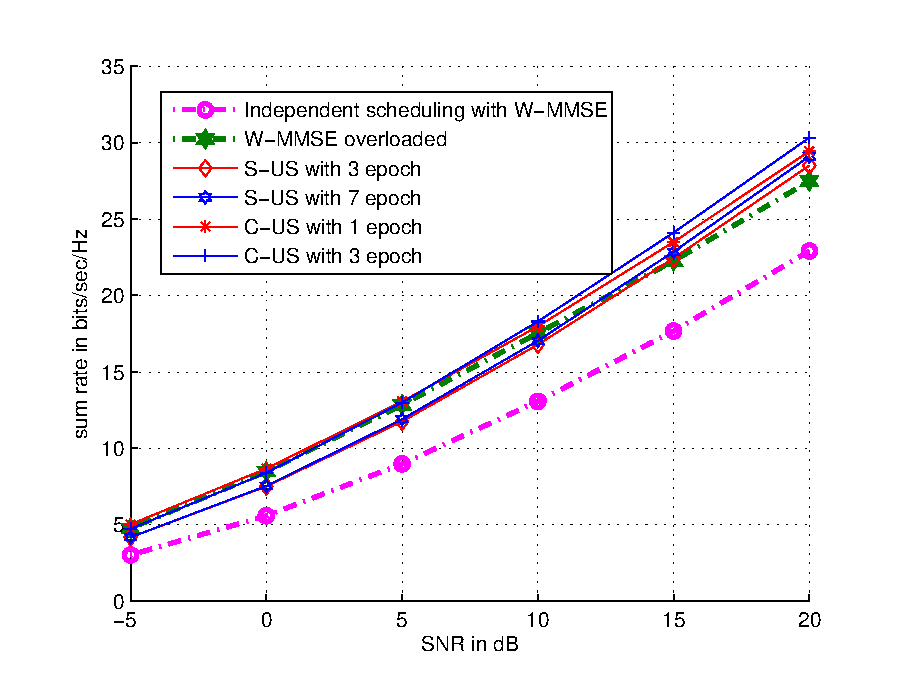
\includegraphics[width=1.0\columnwidth]{multi-bs-2}
\caption[short]{sum rate for \me{N_\mrm{T} = 4, \, N_\mrm{B} = 3, \, \card{\mc{U}_k} = 10}, \, K = 30}
\label{multi-bs-f2}
\vskip -0.1in
\end{figure}

Fig. \ref{multi-bs-f1} compares the performance of the proposed scheduling schemes. The \ac{DoF} available at each \ac{BS} is \me{N_\mrm{T} = 4} which is shared across \ac{BS}s to get \me{\mu} interference-free user streams at each \ac{BS}. The \ac{C-US} scheme performs better in comparison with the other schemes, since the users are shared across the coordinating \ac{BS}s. The sum rate achieved by \ac{C-US} scheme is evidently better than the equivalent near-optimal coordinated \ac{W-MMSE} scheme which performs both \ac{BS} and user assignment jointly. In the static user assignment case, \ac{S-US} scheme performs noticeably better than the overloaded \ac{W-MMSE} scheme at the high \ac{SNR} regime. The gain of the \ac{C-US} scheme over the \ac{S-US} scheme diminishes as the number of users in the system increases to cover all possible channel realizations within the statically assigned users. The precoder design complexity is reduced with limited user set provided by the scheduling schemes. Similar performance can be achieved using \ac{ZF}-\ac{BF} based precoding scheme at the high \ac{SNR} scheme by exploiting the \ac{MU} diversity. The selection of linearly independent users supports \ac{ZF}-\ac{BF} scheme to perform as close to near-optimal \ac{W-MMSE} design.

Fig. \ref{multi-bs-f2} shows the performance of the proposed schemes when the antennas \me{N_\mrm{T}} at each \ac{BS} is not equal to the integer multiple of \me{N_\mrm{B}}. The number of users shared equally among each \ac{BS} are given by \me{\lfloor \, \sfrac{N_\mrm{T}}{N_\mrm{B}} \, \rfloor}. The additional users as given by \me{\mod (N_\mrm{T},N_\mrm{B})} are shared across \ac{BS}s randomly to improve the multiplexing gain. The users are divided as \me{\lfloor \, \sfrac{N_\mrm{T}}{N_\mrm{B}} \, \rfloor + 1} for randomly chosen \me{\mod (N_\mrm{T},N_\mrm{B})} \ac{BS}s and the remaining \ac{BS}s with \me{\lfloor \, \sfrac{N_\mrm{T}}{N_\mrm{B}} \, \rfloor} users at a scheduling instant.

\begin{figure}
\centering
\includegraphics[width=1.0\columnwidth]{multi-bs-3}
\caption[short]{Iterative performance with \me{N_\mrm{T} = 4, \, N_\mrm{B} = 2, \, \card{\mc{U}_k} = 10}, \, K = 20}
\label{multi-bs-f3}
\vskip -0.2in
\end{figure}
The Fig. \ref{multi-bs-f3} portrays the performance improvement of the proposed scheduling schemes over multiple epochs. At each epoch, the sum rate is increased monotonically, for example, \ac{S-US} scheme achieves \me{\approx 2.5} bits by performing multiple epochs. The convergence of the \me{\mc{S}_b \fall b \inm \mc{B}} is not guaranteed to be globally optimal, since the metric used is based on null space projections which itself varies based on the chosen users channel vectors. The complexity reduction of the proposed schemes along with the precoder design is of significant importance, since the precoders are designed for the scheduled users only instead doing for all users in the overloaded \ac{W-MMSE} scenario.


